% figure1_chipflow_v4.tex — COMPACT MINIMAL variant of v1.
% (a) pikv workflow (unchanged from v1).
% (b) 3-column matrix, stripped down:
%     - Reduced chip counts (GPU 5->5+3, Host 10->7).
%     - No column titles, no tier labels (color carries meaning).
%     - Smaller RepairKV pill (\scriptsize, narrower).
%     - Tiny signal-s arrow.
%     - Total panel-(b) height ~3 cm.
% Shared preamble for standalone Figure 1 variants.
\documentclass[border=8pt,tikz]{standalone}
\usepackage{amsmath}
\usepackage{amssymb}
\usepackage{tikz}
\usetikzlibrary{arrows.meta,positioning,calc,fit,shapes.geometric,backgrounds}
\usepackage{xcolor}
\usepackage[T1]{fontenc}
\usepackage{mathptmx}
\newcommand{\repairkv}{\textsc{RepairKV}}
\newcommand{\bbase}{\ensuremath{B_{\mathrm{base}}}}
\newcommand{\bmatch}{\ensuremath{B_{\mathrm{match}}}}

\begin{document}
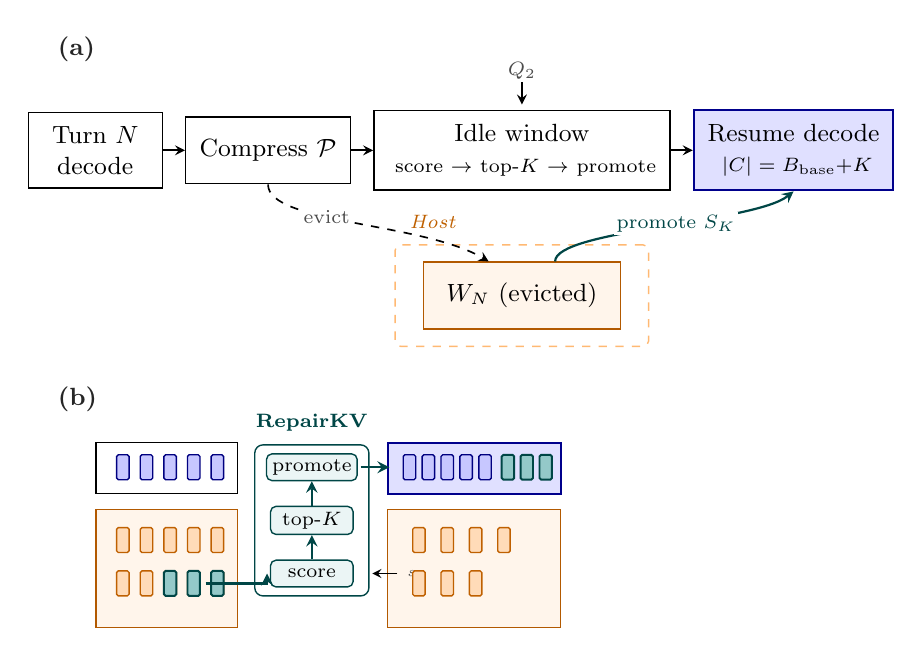
\begin{tikzpicture}[
  >=latex, line width=0.4pt,
  font=\small,
  box/.style={draw=black, fill=white, line width=0.5pt,
              inner sep=5pt, align=center, minimum height=0.85cm},
  active/.style={box, fill=blue!12, draw=blue!55!black, line width=0.7pt},
  store/.style={box, fill=orange!8, draw=orange!70!black},
  arr/.style={->, line width=0.6pt, draw=black, >=stealth},
  promarr/.style={->, line width=0.8pt, draw=teal!55!black, >=stealth},
  arrlabel/.style={font=\scriptsize, text=black!70, fill=white, inner sep=1pt},
  groupbox/.style={draw=orange!55, dashed, line width=0.5pt, rounded corners=2pt},
  grouplabel/.style={font=\scriptsize\itshape, text=orange!75!black},
  panellabel/.style={font=\bfseries\small, text=black!85},
  chip/.style={rounded corners=0.6pt, minimum width=4.5pt, minimum height=9pt,
               inner sep=0pt, line width=0.5pt},
  gpuchip/.style={chip, draw=blue!50!black, fill=blue!22},
  hostchip/.style={chip, draw=orange!75!black, fill=orange!28},
  promchip/.style={chip, draw=teal!55!black, fill=teal!42, line width=0.7pt},
  rkvmod/.style={draw=teal!55!black, fill=teal!8, line width=0.5pt,
                 rounded corners=2pt, inner sep=2pt, align=center,
                 font=\scriptsize, minimum width=1.05cm, minimum height=0.34cm},
  bigpromarr/.style={->, line width=0.9pt, draw=teal!55!black, >=stealth}
]
  % =================================================================
  % Panel (a) — unchanged
  % =================================================================
  \node[panellabel, anchor=south west] at (0, 4.4) {(a)};

  \node[box, minimum width=1.7cm] (dN) at (0.6, 3.4) {Turn $N$\\decode};
  \node[box, minimum width=1.6cm, right=8pt of dN] (cmp) {Compress~$\mathcal{P}$};
  \node[box, minimum width=2.5cm, right=8pt of cmp] (idle)
       {Idle window\\{\scriptsize{} score~$\to$~top-$K$~$\to$~promote}};
  \node[active, minimum width=1.9cm, right=8pt of idle] (resume)
       {Resume decode\\{\scriptsize{} $|C|=\bbase{+}K$}};

  \draw[arr] (dN) -- (cmp);
  \draw[arr] (cmp) -- (idle);
  \draw[arr] (idle) -- (resume);

  \draw[arr] ([yshift=10pt]idle.north) -- ([yshift=2pt]idle.north);
  \node[arrlabel, anchor=south] at ([yshift=10pt]idle.north) {$Q_2$};

  \node[store, minimum width=2.5cm, below=0.9cm of idle] (wn) {$W_N$ (evicted)};
  \node[groupbox, fit=(wn), inner xsep=10pt, inner ysep=6pt] (hgroup) {};
  \node[grouplabel, anchor=south west]
       at ([xshift=2pt, yshift=2pt]hgroup.north west) {Host};

  \draw[arr, dashed]
       (cmp.south) .. controls ([yshift=-0.5cm]cmp.south)
                              and ([yshift=0.5cm]wn.north west) ..
       ([xshift=-12pt]wn.north)
       node[arrlabel, pos=0.4] {evict};

  \draw[promarr]
       ([xshift=12pt]wn.north) .. controls ([xshift=12pt, yshift=0.4cm]wn.north)
                                          and ([xshift=-0.5cm, yshift=-0.4cm]resume.south) ..
       (resume.south)
       node[arrlabel, text=teal!55!black, pos=0.55] {promote~$S_K$};

  % =================================================================
  % Panel (b) — COMPACT 3-column matrix
  % Vertical extent: y = -0.3 (top of GPU) to y = -3.3 (bottom of host) ~ 3 cm
  % Column 1 (before): x=0.6..2.4   width 1.8
  % Column 2 (middle): x=2.7..4.0   width 1.3 (smaller pill)
  % Column 3 (after):  x=4.3..6.5   width 2.2
  % =================================================================
  \node[panellabel, anchor=south west] at (0, -0.05) {(b)};

  % GPU rows: height 0.65 cm
  \node[box, minimum width=1.8cm, minimum height=0.65cm,
        anchor=north west] (gpuB) at (0.6, -0.30) {};
  \node[active, minimum width=2.2cm, minimum height=0.65cm,
        anchor=north west] (gpuA) at (4.3, -0.30) {};

  % Host rows: height ~1.4 cm (2 sub-rows of chips)
  \node[store, minimum width=1.8cm, minimum height=1.5cm,
        anchor=north west] (hostB) at (0.6, -1.15) {};
  \node[store, minimum width=2.2cm, minimum height=1.5cm,
        anchor=north west] (hostA) at (4.3, -1.15) {};

  % --- Middle column: RepairKV pill (smaller) ---
  % Center column x ~ 3.35
  \node[rkvmod, anchor=center] (mpromote) at (3.35, -0.625) {promote};
  \node[rkvmod, anchor=center] (mselect)  at (3.35, -1.30)  {top-$K$};
  \node[rkvmod, anchor=center] (mscore)   at (3.35, -1.975) {score};
  \draw[promarr] (mscore.north)  -- (mselect.south);
  \draw[promarr] (mselect.north) -- (mpromote.south);

  \node[draw=teal!55!black, line width=0.5pt, rounded corners=3pt,
        fit=(mpromote)(mscore), inner xsep=4pt, inner ysep=3pt] (rkvframe) {};
  \node[font=\scriptsize\bfseries, text=teal!55!black, anchor=south]
       at ([yshift=1pt]rkvframe.north) {\repairkv{}};

  % --- Signal s: small arrow + tiny label, on the right side at score level ---
  \draw[arr, line width=0.45pt]
       ([xshift=10pt]rkvframe.east |- mscore)
       -- ([xshift=1pt]rkvframe.east |- mscore);
  \node[font=\tiny, text=black!70, anchor=west]
       at ([xshift=10pt]rkvframe.east |- mscore) {$s$};

  % --- GPU before: 5 blue chips ---
  % gpuB inner width ~1.8 cm; chip width 4.5pt (~0.16cm) + spacing
  \foreach \i in {1,...,5}{
    \pgfmathsetmacro{\xc}{0.30*\i + 0.05}
    \node[gpuchip] at ([xshift=\xc cm, yshift=-0.325cm]gpuB.north west) {};
  }
  % --- GPU after: 5 blue + 3 teal ---
  \foreach \i in {1,...,5}{
    \pgfmathsetmacro{\xc}{0.24*\i + 0.05}
    \node[gpuchip] at ([xshift=\xc cm, yshift=-0.325cm]gpuA.north west) {};
  }
  \foreach \i in {1,2,3}{
    \pgfmathsetmacro{\xs}{0.24*5 + 0.24*\i + 0.10}
    \node[promchip] at ([xshift=\xs cm, yshift=-0.325cm]gpuA.north west) {};
  }

  % --- Host before: 2 sub-rows of 5 chips = 10 total; 3 teal candidates at end of row 2 ---
  \foreach \i in {1,...,5}{
    \foreach \r in {0,1}{
      \pgfmathsetmacro{\xh}{0.30*\i + 0.05}
      \pgfmathsetmacro{\yh}{-0.40 - 0.55*\r}
      \node[hostchip] at ([xshift=\xh cm, yshift=\yh cm]hostB.north west) {};
    }
  }
  % Convert last 3 chips on row 2 to teal (over-paint)
  \foreach \i in {3,4,5}{
    \pgfmathsetmacro{\xh}{0.30*\i + 0.05}
    \node[promchip] (hostTeal\i) at ([xshift=\xh cm, yshift=-0.95cm]hostB.north west) {};
  }
  % anchor used for arrow
  \coordinate (hostTealMid) at ([xshift=1.40cm, yshift=-0.95cm]hostB.north west);

  % --- Host after: 7 chips (3 fewer) ---
  % Row 1: 4 chips, Row 2: 3 chips
  \foreach \i in {1,...,4}{
    \pgfmathsetmacro{\xh}{0.36*\i + 0.05}
    \node[hostchip] at ([xshift=\xh cm, yshift=-0.40cm]hostA.north west) {};
  }
  \foreach \i in {1,...,3}{
    \pgfmathsetmacro{\xh}{0.36*\i + 0.05}
    \node[hostchip] at ([xshift=\xh cm, yshift=-0.95cm]hostA.north west) {};
  }

  % --- Flow arrows: short, row-level ---
  % Host candidates -> score (entering pill from left)
  \draw[bigpromarr] (hostTealMid) -- ([xshift=-1pt]mscore.west |- hostTealMid)
                                  -- ([xshift=-1pt]mscore.west);
  % promote -> GPU after (left edge)
  \draw[bigpromarr] ([xshift=1pt]mpromote.east)
                    -- ([xshift=1pt]mpromote.east -| gpuA.west);
\end{tikzpicture}
\end{document}
